\section{Peuplement semi-automatique d'ontologies métiers}

Problématique du bruit

Nous avons développé une application web, Curiositext, permettant à un utilisateur non expert de visualiser les résultats de Word2Vec et de peupler semi-automatiquement une ontologie métier. Celle-ci est indépendante de l'architecture de l'application ce qui permet d'utiliser CuriosiText pour des cas d'usage très divers, sans dépendre d'un domaine spécifique. Dans un premier temps, l'utilisateur est invité à charger un corpus texte local ou peut effectuer une requête à l'aide d'Elastic Search pour récupérer des données distantes. Il peut ensuite appliquer Word2Vec sur ses données. Les paramètres de base de la méthode sont paramétrables à savoir : la dimension des vecteurs, la taille de la fenêtre, la fréquence minimale d'apparition d’un terme pour l’apprentissage, le modèle (CBOW ou Skip-Gram) et le nombre d’itérations.

\begin{figure}[tb]
    \begin{center}
        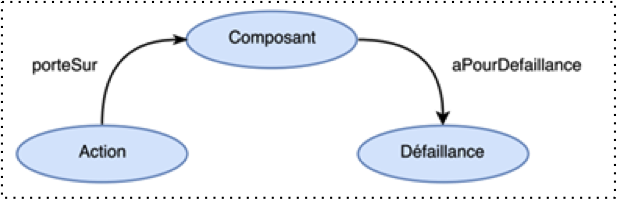
\includegraphics[width=6cm]{figures/ontMetier}
    \end{center}
    \caption{Ontologie métier}\label{fig:metier}
\end{figure}

L'utilisateur accède ensuite à la troisième partie de l'application à savoir le peuplement d'une ontologie. Il doit charger l’ontologie métier (fig \ref{fig:metier}) développée en amont à peupler. Pour ce faire, nous avons mis en place un scénario de peuplement de l'ontologie finale illustré ici par la requête du terme "changement".
Pour aider au peuplement de l'ontologie, une ontologie linguistique (fig \ref{ling} a été intégrée dans l'application. L'utilisateur doit renseigner pour le terme requêté sa classe lexicale (Terme\_Canonique) et sa classe métier (Action).

\begin{figure}[tb]
    \begin{center}
        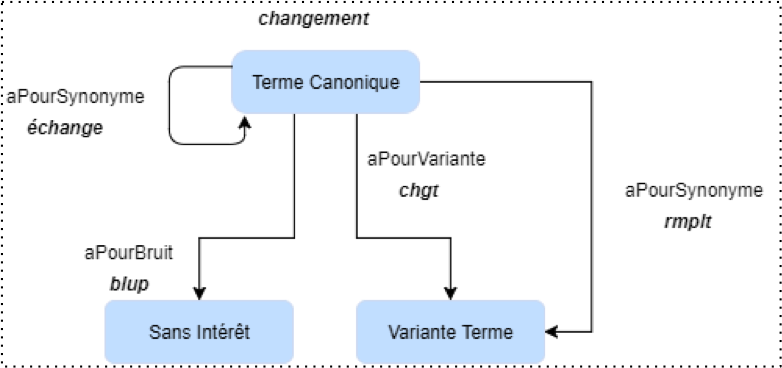
\includegraphics[width=8cm]{figures/ontLing}
    \end{center}
    \caption{Ontologie linguistique}\label{fig:ling}
\end{figure}



L'intérêt d'utiliser directement un entrepôt RDF comme backend de l'application nous permet de bénéficier, en plus des capacités de requêteage et de stockage, les possibilités de raisonnement définies lors de la création des ontologies. En effet, les déductions effectuées par l'entrepôt permmettent à l'interface de ne fournir que les informations minimales à celui-ci : il se charge de compléter celles-ci à l'aide de la formalisation OWL (RL)\cite{owlprofiles} définie dans les ontologies. Par exemple, le fait d'ajouter un lien de synonymie ou de variance dans les données va permmettre éventuellement de déduire l'appartenance d'un individu à une classe métier (ici Action) grâce à l'axiome ci-dessous\footnote{Notons que nous sommes obligé de dupliquer ce type d'axiome pour chaque classe concernée.
} :
$$
\begin{array}{ll}
\exists  \ \texttt{aPourSynonyme} .  \texttt {Action}  \sqcup \exists  \ \texttt{aPourVariante} .  \texttt {Action}
\sqsubseteq    \texttt{Action}
\end{array}
$$
En logique de description, cela signifie que tout individu qui a un synonyme ou une variante dans la classe Action appartient à la classe Action lui-même. Nous faisons la même chose pour les classes Composant et Defaillance, la logique du premier ordre ne nous permettant pas d'écrire des axiomes sur des ensembles de classes.
L'interface ne fait que qu'ajouter ou retirer des triplés RDF élémentaires, l'intelligence de l'entrepôt se charge de faire les mises à jour déclenchées par le raisonnement et éventuellement de détecter des incohérences dans les données.
